\chapter{Framework Design, Description, and Implementation}\label{ch: Framework Design}
% The initial document describing the framework's design for instantiating and running a multiagent system described using an ontology, and possibly several iterations of it, as it is being refined.

% Developed framework that allows the user to instantiate agents and run a multiagent system based on the description of the desired system using the developed ontology for describing and instantiating a multiagent system.

The main objective of the \magoontologyname framework
\lookAt{\cref{fig: ontology framework template}}
is to provide a medium for converting a \ac{MAS} model defined using the related \magoontologyname ontology into a template for implementing the modelled system using \ac{SPADE} library of Python. The rendered implementation template is not expected to include all the details that might be needed to run the finished system of agents. Still, it is planned to provide the initial implementation requirements of the modelled system. Including all the implementation details in the ontology might prove to be too cumbersome and taxing for the modelling process.

The framework is expected to translate the necessary elements of the ontology to classes, objects, and instances where applicable and provide the rest of the ontology knowledge to agents translated into applicable data types.

\begin{figure}
    \centering
    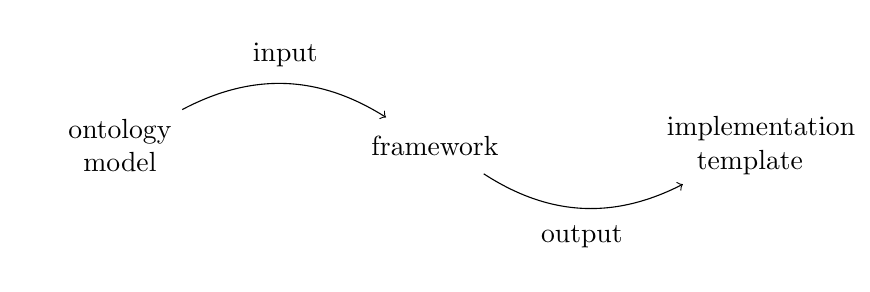
\begin{tikzpicture}
    [
        every node/.style={minimum height=2em, text width=6em, align=center},
        every path/.style={->},
    ]
  % Nodes
  \node [] (O) at (-4,0) {ontology model};
  \node [] (F) at (0,0) {framework};
  \node [] (I) at (4,0) {implementation template};

  % Connections
  \draw [] (O) to[bend left] node[midway, above] {input} (F);
  \draw [] (F) to[bend right] node[midway, below] {output} (I);
\end{tikzpicture}

    \caption{\magoontologyname framework workflow}
    \label{fig: ontology framework template}
\end{figure}



\section{Framework Design and Description}

The key requirements of the framework are, therefore, the following.

\begin{itemize}
    \item \mintedInline{Agent} subconcepts must be translatable into classes extending the \mintedInline{Agent} class of \ac{SPADE}. Every \ac{SPADE} agent must connect to an \ac{XMPP} server in order to be able to communicate with other agents. To connect to an \ac{XMPP} server, the agent must have a \mintedInline{name} and the address of the \ac{XMPP} server it is connecting to. Furthermore, individuals of the \mintedInline{Agent} must be translated into objects of the appropriate agent class defined in \ac{SPADE}.

    \item \mintedInline{Behaviour} individuals can usually be found in the extension of one of the six subconcepts of the \mintedInline{Behaviour} concept. These individuals must be implemented by extending the appropriate class defined in \ac{SPADE}. Since behaviour implementations highly depend on the intended use of the system and the agents therein, various details of the actual implementation of behaviour are not planned to be a part of the implementation template generated by this framework. Therefore, \mintedInline{Behaviour} individuals are expected to be translated only to the point of a defined behaviour class that can be instantiated by individual agents. One key observation is that agents, by default, know no behaviours. Instead, they learn about the available behaviours by playing, i.e. enacting, different \mintedInline{Role} individuals. Individuals of the \mintedInline{Role} concept are planned to be implemented in a way that is accessible by an agent, e.g. as a value of their internal attribute.

    \item By default, \ac{SPADE} agents communicate using the \ac{XMPP} protocol that requires a connection to an active \ac{XMPP} server. Therefore, every agent must be connected to exactly one individual of the \mintedInline{Agent Host Server} concept. This concept must provide the host the \mintedInline{Agent} individual has to connect to, while the other part of the \ac{JID}, the name, is provided by the \mintedInline{Agent} individual itself.
\end{itemize}

The \magoontologyname ontology provides the basic concepts for the framework to translate. However, the framework must be able to work with additional subconcepts introduced to the \mintedInline{Agent} concept. This requirement stems from the need to allow the system modeller to create agent classes and their individual agents. Furthermore, the \magoontologyname framework must work with individuals, even though treating individuals of \mintedInline{Agent} concept is expected to be different to how individuals of the \mintedInline{Behaviour} concept are treated; individual behaviours should be implemented as behaviour classes that will be instantiated by individual agents, while individual agents are instances of the applicable \mintedInline{Agent} class. Ultimately, extending the framework to include additional concepts that may be introduced to the related ontology in the future should not be extremely difficult.

\primjer{
    Subconcepts of the \mintedInline{Agent} concept can be \mintedInline{Agent Factory} and\\\mintedInline{Agent Recipe} in the domain where recipe agents consume a subset of the set of services provided by factory agents, which is, in turn, a subset of the system-wide set of possible services. 
}{Subconcepts to the \mintedInline{Agent} concept}

Finally, the framework should be implemented to provide the user with its functionality without requiring extensive programming or \ac{SPADE} knowledge. In other words, the framework must be easy to run and provide the results straightforwardly.



\section{Framework Implementation}

The framework was developed in stages; each focused on one of the concepts that must be translated into the implementation template. Several Python classes are developed, to help the translation process.

\newthought{Thing}
\marginnote{\mintedInline{Thing}}%
was the initial entity to be developed. The main idea of the \mintedInline{Thing} class was to create a set of methods and properties that will be common to all the classes used for translating the ontology to the appropriate implementation template. The \mintedInline{Thing} class is to be extended by the other classes participating in the translation process. Therefore, the class implementation includes the following key elements.

\begin{itemize}
    \item Some basic values as class properties are stored that are planned to be available to and used by the other classes.

    \item Common methods for the following purposes are provided:

    \begin{itemize}
        \item 
        \marginnote[2px]{\mintedInline{set_implementation_template}}%
        setting up the string template for the resulting implementation template;
        \lookAt{\cref{lst: mago-ag thing set_implementation_template}}%

        \item
        \marginnote[2px]{\mintedInline{render_implementation}}%
        rendering the implementation template via substituting the placeholder values in the implementation string template;
        \lookAt{\cref{lst: mago-ag thing render_implementation}}%

        \item
        \marginnote[2px]{\mintedInline{get_implementation}}%
        retrieving the implementation template if it is already rendered, whenever needed;
        \lookAt{\cref{lst: mago-ag thing get_implementation}}%

        \item
        \marginnote[2px]{\mintedInline{write_implementation_to_file}}%
        writing the rendered implementation template in a file on the local disk.
        \lookAt{\cref{lst: mago-ag thing write_implementation_to_file}}%
    \end{itemize}
\end{itemize}

\begin{listing}
    \mintedFilePython[firstline=64, lastline=71]{Deliverables/Phase 1/Implementation/mago_thing.py}
    \caption{Implementation of the \mintedInline{set_implementation_template} method of the \mintedInline{Thing} class}
    \label{lst: mago-ag thing set_implementation_template}
\end{listing}

\begin{listing}
    \mintedFilePython[firstline=73, lastline=88]{Deliverables/Phase 1/Implementation/mago_thing.py}
    \caption{Implementation of the \mintedInline{render_implementation} method of the \mintedInline{Thing} class}
    \label{lst: mago-ag thing render_implementation}
\end{listing}

\begin{listing}
    \mintedFilePython[firstline=90, lastline=96]{Deliverables/Phase 1/Implementation/mago_thing.py}
    \caption{Implementation of the \mintedInline{get_implementation} method of the \mintedInline{Thing} class}
    \label{lst: mago-ag thing get_implementation}
\end{listing}

\begin{listing}
    \mintedFilePython[firstline=98, lastline=117]{Deliverables/Phase 1/Implementation/mago_thing.py}
    \caption{Implementation of the \mintedInline{write_implementation_to_file} method of the \mintedInline{Thing} class}
    \label{lst: mago-ag thing write_implementation_to_file}
\end{listing}



\newthought{Agent}
\marginnote{\mintedInline{Agent}}%
was the following entity to be developed. The \mintedInline{Agent} class is developed to be the extension of the \mintedInline{Thing} class. In addition to the method for setting up the rendering string template, the \mintedInline{Agent} class features three other methods with the following functionalities.

\begin{itemize}
    \item
    \marginnote[2px]{\mintedInline{get_related_roles_and_behaviours}}%
    In order to provide the \mintedInline{Agent} individual with the knowledge of roles and the behaviours they enable, role and behaviour combinations are retrieved, constrained to the roles available to the individual agent.
    \lookAt{\cref{lst: mago-ag agent get_related_roles_and_behaviours}}%

    \item
    \marginnote[2px]{\mintedInline{render_agent_instantiation}}%
    \ac{SPADE} agents are instances of their respective agent classes. Therefore, the \mintedInline{Agent} class provides the method for rendering a part of the agent instantiation code.
    \lookAt{\cref{lst: mago-ag agent render_agent_instantiation}}%

    \item
    \marginnote[2px]{\mintedInline{render_agent_import}}%
    Since agent individuals may pertain to custom agent subconcepts, it is necessary to allow their successful translation to implementation templates. This is why the \mintedInline{Agent} class provides the method for rendering the import statement for a particular agent.
    \lookAt{\cref{lst: mago-ag agent render_agent_import}}%
\end{itemize}

\begin{listing}
    \mintedFilePython[firstline=93, lastline=111]{Deliverables/Phase 1/Implementation/mago_agent.py}
    \caption{Implementation of the \mintedInline{get_related_roles_and_behaviours} method of the \mintedInline{Agent} class}
    \label{lst: mago-ag agent get_related_roles_and_behaviours}
\end{listing}

\begin{listing}
    \mintedFilePython[firstline=113, lastline=125]{Deliverables/Phase 1/Implementation/mago_agent.py}
    \caption{Implementation of the \mintedInline{render_agent_instantiation} method of the \mintedInline{Agent} class}
    \label{lst: mago-ag agent render_agent_instantiation}
\end{listing}

\begin{listing}
    \mintedFilePython[firstline=127, lastline=134]{Deliverables/Phase 1/Implementation/mago_agent.py}
    \caption{Implementation of the \mintedInline{render_agent_import} method of the \mintedInline{Agent} class}
    \label{lst: mago-ag agent render_agent_import}
\end{listing}



\newthought{Behaviour}
\marginnote{\mintedInline{Behaviour}}%
is the next entity to be developed. The \mintedInline{Behaviour} class is developed to be the extension of the \mintedInline{Thing} class as well.

Since all the \mintedInline{Behaviour} individuals are ultimately individuals of the \mintedInline{Behaviour} concept in the ontology, and their further classification is performed via the applied reasoning processes since their respective subconcepts are implemented as defined classes, their specific type (i.e. cyclic, periodic, one-shot, timeout, finite state machine, or state) is determined
\marginnote{\mintedInline{determine_behaviour_type}}%
using a specific method of the \mintedInline{Behaviour} class based on their individual's data property values.
\lookAt{\cref{lst: mago-ag behaviour determine_behaviour_type}}%

\mintedInline{Finite State Machine Behaviour} is the most complex behaviour to translate. Even though the behaviour class is implemented in the same manner the other behaviour classes are implemented, the \ac{FSM} behaviour must have all the states
\marginnote{\mintedInline{get_fsm_states}}%
and their transitions set up too. The process of setting up the initial state, the other states,
\lookAt{\cref{lst: mago-ag behaviour get_fsm_states}}%
and their respective transitions requires traversing through the individuals of the ontology. Therefore, an extra method
\marginnote{\mintedInline{render_fsm_implementation}}%
was developed as a part of the behaviours of the \mintedInline{Finite State Machine Behaviour} concept
\lookAt{\cref{lst: mago-ag behaviour render_fsm_implementation}}%
that will be used to set up the behaviour in runtime.

\begin{listing}
    \mintedFilePython[firstline=17, lastline=35]{Deliverables/Phase 1/Implementation/mago_behaviour.py}
    \caption{Implementation of the \mintedInline{determine_behaviour_type} method of the \mintedInline{Behaviour} class}
    \label{lst: mago-ag behaviour determine_behaviour_type}
\end{listing}

\begin{listing}
    \mintedFilePython[firstline=37, lastline=58]{Deliverables/Phase 1/Implementation/mago_behaviour.py}
    \caption{Implementation of the \mintedInline{get_fsm_states} method of the \mintedInline{Behaviour} class}
    \label{lst: mago-ag behaviour get_fsm_states}
\end{listing}

\begin{listing}
    \mintedFilePython[firstline=60, lastline=98]{Deliverables/Phase 1/Implementation/mago_behaviour.py}
    \caption{Implementation of the \mintedInline{render_fsm_implementation} method of the \mintedInline{Behaviour} class}
    \label{lst: mago-ag behaviour render_fsm_implementation}
\end{listing}



\newthought{Strategy}
\marginnote{\mintedInline{Strategy}}%
concepts are the last entities to be developed. The \mintedInline{Plan} class is developed to be the extension of the \mintedInline{Thing} class again.

The goal of translating the strategy-related concepts into the implementation template is to provide agent instances with the knowledge from the ontology in a way that is more Python-friendly. Furthermore, by removing the necessity of having the ontology available to agent instances, the implementation template is rendered as a more independent system. This decision introduces some other constraints, though, such as no reasoning over the knowledge rendered as data. On the other hand, access to an ontology can still be given to an agent using the \mintedInline{Knowledge Artefact} concept.

The strategy-related concepts are translated
\marginnote{\mintedInline{get_plan_action_behaviour_objective}}%
using a single method that translates the related \mintedInline{Plan}, \mintedInline{Action}, \mintedInline{Behaviour}, and \mintedInline{Objective} individuals into a Python dictionary
\lookAt{\cref{lst: mago-ag plan get_plan_action_behaviour_objective}}%
retaining their respective connections.

\begin{listing}
    \mintedFilePython[firstline=8, lastline=65]{Deliverables/Phase 1/Implementation/mago_plan.py}
    \caption{Implementation of the \mintedInline{get_plan_action_behaviour_objective} method of the \mintedInline{Plan} class}
    \label{lst: mago-ag plan get_plan_action_behaviour_objective}
\end{listing}



\newthought{Knowledge artefact}
individuals are provided to the connected agents via their \acp{URI}.
\marginnote{\mintedInline{get_related_knowledge_artefact_uris}}%
Each agent is provided with a property of data type dictionary,
\lookAt{\cref{lst: mago-ag aux get_related_knowledge_artefact_uris}}%
consisting of artefacts' names and \acp{URI}.

\begin{listing}
    \mintedFilePython[firstline=32, lastline=56]{Deliverables/Phase 1/Implementation/aux.py}
    \caption{Implementation of the \mintedInline{get_related_knowledge_artefact_uris} function}
    \label{lst: mago-ag aux get_related_knowledge_artefact_uris}
\end{listing}



\newthought{Workspace}
is the last entity to be developed. The Python class for this concept is used to perform most of the necessary rendering and writing to file operations of the related concepts and individuals. This class contains all the methods necessary for getting all the data from the ontology and rendering the implementation templates. While writing rendered implementation templates to files is mostly performed by calling the related methods of the \mintedInline{Thing} class, the following more interesting methods are used to retrieve data from the ontology containing the modelled \ac{MAS}:

\begin{itemize}
    \item \mintedInline{read_agents_from_ontology} implements
    \lookAt[4px]{\cref{lst: mago-ag workspace read_agents_from_ontology}}%
    how to read the ontology, retrieve the most important data related to agents, and prepare those data for rendering agent implementation templates;
    
    \item \mintedInline{render_behaviours_from_ontology} renders
    \lookAt[4px]{\cref{lst: mago-ag workspace render_behaviours_from_ontology}}%
    behaviour implementation templates based on their ontology data
    
    \item \mintedInline{read_plan_from_ontology} takes
    \lookAt[4px]{\cref{lst: mago-ag workspace read_plan_from_ontology}}%
    all the \mintedInline{Plan} individuals and renders their related data as a Python dictionary.
\end{itemize}

\begin{listing}
    \mintedFilePython[firstline=25, lastline=43]{Deliverables/Phase 1/Implementation/mago_workspace.py}
    \caption{Implementation of the \mintedInline{read_agents_from_ontology} method of the \mintedInline{Workspace} class}
    \label{lst: mago-ag workspace read_agents_from_ontology}
\end{listing}

\begin{listing}
    \mintedFilePython[firstline=45, lastline=69]{Deliverables/Phase 1/Implementation/mago_workspace.py}
    \caption{Implementation of the \mintedInline{render_behaviours_from_ontology} method of the \mintedInline{Workspace} class}
    \label{lst: mago-ag workspace render_behaviours_from_ontology}
\end{listing}

\begin{listing}
    \mintedFilePython[firstline=71, lastline=88]{Deliverables/Phase 1/Implementation/mago_workspace.py}
    \caption{Implementation of the \mintedInline{read_plan_from_ontology} method of the \mintedInline{Workspace} class}
    \label{lst: mago-ag workspace read_plan_from_ontology}
\end{listing}



\newthought{Translation}
script
\lookAt{\cref{lst: mago-ag translate}}%
is the very last element that must be added to the mix, in order to make the framework easily runnable and usable. The main translation script starts by reading the ontology using the \mintedInline{owlready2} library, then instantiates the \mintedInline{Workspace} object, and by calling the \mintedInline{write_implementation_to_disk} of the instantiated \mintedInline{World} object finally runs the translation process. Thus, the ontology is consulted, the necessary string templates are rendered, and the implementation template is written to respective files.

\begin{listing}
    \mintedFilePython[]{Deliverables/Phase 1/Implementation/translate.py}
    \caption{The main script of the framework}
    \label{lst: mago-ag translate}
\end{listing}
